\documentclass[a4paper,12pt]{article}

\usepackage[T1]{fontenc}
\usepackage[utf8]{inputenc}

\usepackage{amssymb, amsmath, amsthm}
\usepackage[output-decimal-marker={,},
            group-separator={},
            separate-uncertainty=true,
            scientific-notation=true]{siunitx}

\usepackage{subfig}
\usepackage{pgfplots}
\usepackage{pgfplotstable}
\pgfplotsset{compat=1.16}
\usetikzlibrary{arrows.meta}
\usetikzlibrary{backgrounds}
\usepackage{csvsimple}

\usepackage[swedish]{babel}
\usepackage{lipsum}
\usepackage{parskip}

\newcommand*{\dd}{\mathrm{d}}

\begin{document}

\begin{titlepage}
  \centering
  \vspace{10cm}
  {\Huge Torsionspendel \\}
  \vspace{2cm}
  {\Large TFYA81 -- Experimentell problemlösning \\}
  \vspace{0.8em}
  {\Large Laborationsrapport}
  \vfill

  {
    \textsc{Philip Holm} -- phiho621 \\
    \textsc{Gustav Sörnäs} -- gusso230 \\
    \vspace{2cm}
    Teknisk fysik och elektroteknik (Y) \\
    Linköpings universitet\\\today{}\\Version 2
  }

  % Bottom of the page
  %{\large \today\par}
\end{titlepage}

\pagenumbering{gobble}
\section*{Sammanfattning}

En modell för periodtiden för en torsionspendel med påhängda vikter har tagits
fram via experiment och beräkningar:

\begin{equation*}
  T = \frac{c_2 \sqrt{l(ma^2 + c_1)}}{d^2 \sqrt{G}},
\end{equation*}

där $T$ är periodtiden, $l$ och $d$ är trådens längd respektive diameter, $m$ är
de påhängda vikternas massa, $a$ är längden mellan pendelns centrum och
ytterkanten på de påhängda vikterna och $G$ är trådens skjuvmodul. $c_1$
uppmättes till \SI{8.93(8)e-4}{\kilogram \meter \squared} och $c_2$ till
\num{29.68(6)}.

\clearpage

\tableofcontents
\listoffigures
\listoftables
\clearpage

\pagenumbering{arabic}

\section{Inledning}

Syftet med laborationen var att ta fram en modell för periodtiden för en stång i
en torsionspendel med påhängda vikter som berodde på trådens längd, diameter,
massan av de påhängda vikterna samt hur långt ut på stången vikterna sattes.

\section{Metod}

\begin{figure}
\centering
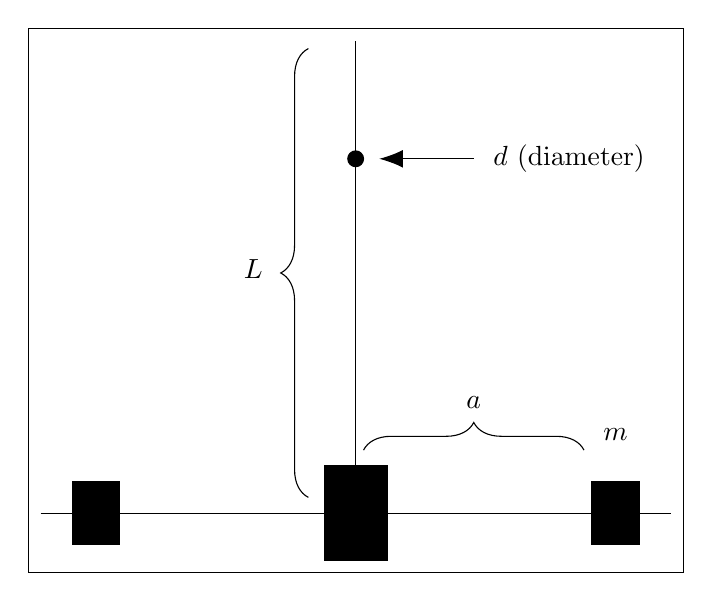
\begin{tikzpicture}[framed]
  \draw ( 0,0) -- (0,6);
  \draw (-4,0) -- (4,0);
  \draw [fill=black] (-0.4,-0.6) rectangle (0.4,0.6);
  \draw [fill=black] (-3.6,-0.4) rectangle (-3,0.4);
  \draw [fill=black] (3.0, -0.4) rectangle (3.6,0.4);
  \node at (3.3,1.0) {$m$};
  \draw [decoration={brace,amplitude=10pt},decorate] (0.1,0.8) -- (2.9,0.8);
  \node at (1.5, 1.4) {$a$};
  \draw [decoration={brace,amplitude=10pt},decorate] (-0.6,0.2) -- (-0.6,5.9);
  \node at (-1.3, 3.1) {$L$};
  \draw [fill=black](0,4.5) circle (0.1cm);
  \draw [-{Latex[length=3mm]}] (1.5,4.5) -- (0.3,4.5);
  \node at (2.71,4.5) {$d$ (diameter)};
\end{tikzpicture} 
\caption{Laborationens uppställning}
\label{fig:uppställning}
\end{figure}

%\subsection{Experimentets utförande}
En metalltråd fästes med hjälp av en tving-liknande klämma i ena änden och läts
i andra änden hänga fritt (se figur~\ref{fig:uppställning}). I den fria änden fästes
mitten av en stång med en insexnyckel. På stångens båda sidor skruvades vikter
på med lika avstånd från mittpunkten av stången. Vid vardera mätning roterades
stången en bit och läts sedan pendla fritt. Pendeltiden mättes för tio
pendelutslag åt gången för att minska osäkerheten.

\subsection{Ingående variabler}

\begin{table}[h!]
  \caption{Storheter}
  \label{tab:storheter}
  \begin{tabular} {| l | l | l | l |}
    \hline
    \textbf{Beskrivning} & \textbf{Variabel} & \textbf{Enhet} & \textbf{Dimension} \\\hline
    Trådens längd & $l$ & [m] & L \\\hline
    Trådens diameter & $d$ & [m] & L \\\hline
    Viktens massa & $m$ & [kg] & M \\\hline
    Viktens avstånd från mitten & $a$ & [m] & L \\\hline
    Trådens skjuvmodul & $G$ & [Pa] $=$ [kg $\mathrm{m}^{-1}$ $\mathrm{s}^{-2}$] & M $\mathrm{L}^{-1}$ $\mathrm{T}^{-2}$ \\\hline
    Pendeltiden & $T$ & [s] & T \\\hline
  \end{tabular}
\end{table}

Ingående variabler som antogs påverka pendeltiden presenteras i
tabell~\ref{tab:storheter}. Trådens diameter mättes med en mikrometer. Övriga
längder mättes med måttband.  Massan mättes med våg, skjuvmodulerna gavs i
laborationsinstruktionen och tiden mättes med stoppur.

\subsection{Hypotes}

Sambandet antogs i huvudsak vara multiplikativt. Eftersom pendeltiden rimligtvis
inte är 0 när en massa inte hängs på och både $m$ och $a$ påverkas av den
påhängda massan antogs att $m^\gamma$ och $a^\sigma$ adderas med en konstant
$c_1$ med någon okänd dimension [$\si{\kilogram}^\gamma\si{\meter}^\sigma$].
Ekvation~\eqref{eq:hypotes} fördes fram som hypotes.

\begin{equation}
  T = L^\alpha \cdot d^\beta \cdot (m^\gamma \cdot a^\sigma + c_1)^\omega \cdot G^\lambda \cdot c_2
  \label{eq:hypotes}
\end{equation}

\subsection{Dimensionsanalys}

Givet hypotesen ficks följande ekvationssystem gällande exponenterna.

\begin{equation}
  %\left\{
  \begin{array}{rrcc}
    \text{m:} & \hspace{1em} \alpha + \beta + \sigma \omega - \lambda & = & 0 \\
    \text{kg:} & \gamma \omega + \lambda & = & 0 \\
    \text{s:} & 2\lambda & = & 1
  \end{array}
  \label{eq:system}
\end{equation}

$\lambda = \frac{-1}{2}$ antogs som uppenbar. $\alpha$ och $\beta$ ficks sedan genom
linjäriseringar och $\gamma$, $\sigma$ och $\omega$ ficks genom en ansats.

%\clearpage

\section{Resultat}

\subsection{Linjärisering}

19 mätningar (mätserie~1) gjordes där $L$ var den enda variabeln som varierades
varpå följande linjärisering genomfördes.

\begin{align}
  \ln T &= \ln (L^\alpha \cdot d^\beta \cdot (m^\gamma \cdot a^\sigma + c_1)^\omega \cdot G^\lambda \cdot c_2) \nonumber \\
  \ln T &= \ln (L^\alpha) + \ln (d^\beta \cdot (m^\gamma \cdot a^\sigma + c_1)^\omega \cdot G^\lambda \cdot c_2) \nonumber \\
  \ln T &= \alpha \ln L + \ln (d^\beta \cdot (m^\gamma \cdot a^\sigma + c_1)^\omega \cdot G^\lambda \cdot c_2)  \label{eq:lin_La}
\end{align}

Dessutom gjordes 15 mätningar (mätserie~2) där $d$ var den enda variabeln som
varierades och följande linjärisering gjordes.

\begin{align}
  \ln T &= \ln (L^\alpha \cdot d^\beta \cdot (m^\gamma \cdot a^\sigma + c_1)^\omega \cdot G^\lambda \cdot c_2) \nonumber \\
  \ln T &= \ln (d^\beta) + \ln (L^\alpha \cdot (m^\gamma \cdot a^\sigma + c_1)^\omega \cdot G^\lambda \cdot c_2) \nonumber \\
  \ln T &= \beta\ln d + \ln (L^\alpha \cdot (m^\gamma \cdot a^\sigma + c_1)^\omega \cdot G^\lambda \cdot c_2)  \label{eq:lin_db}
\end{align}

Ekvationerna \eqref{eq:lin_La} och \eqref{eq:lin_db} ritades upp
(figur~\ref{fig:lin_La} och figur~\ref{fig:lin_db}).

\begin{figure}
  \begin{tikzpicture}
    \begin{axis} [
      ylabel=$\ln T$,
      xlabel=$\ln L$,
      xmin=-2.1, xmax=-0.9,
      ymin=-0.45, ymax=0.14,
      legend pos = outer north east,
      ]
      \addplot+ [mark=none] {0.4601*x + 0.5066};
      \addlegendentry {$\num[scientific-notation=false]{0.46}x + \num[scientific-notation=false]{0.51}$};
      \addplot+ [only marks,mark=*,color=blue,mark options={fill=blue}] table [col sep=comma, x index=2, y index=3] {data/var_l.csv};
    \end{axis}
  \end{tikzpicture}
  \caption{Linjärisering med avseende på $L$}
  \label{fig:lin_La}
\end{figure}

\begin{figure}
  \begin{tikzpicture}
    \begin{axis} [
      ylabel=$\ln T$,
      xlabel=$\ln d$,
      xmin=-6.45, xmax=-5.95,
      ymin=1.85, ymax=2.65,
      legend pos = outer north east,
      ]
      \addplot+ [mark=none,domain=-7:-5] {-1.897*x - 9.4668};
      \addlegendentry {$\num[scientific-notation=false]{-1.9}x - \num[scientific-notation=false]9.5$};
      \addplot+ [only marks,mark=*,color=blue,mark options={fill=blue}] table [col sep=comma, x index=2, y index=3] {data/var_d.csv};
    \end{axis}
  \end{tikzpicture}
  \caption{Linjärisering med avseende på $d$}
  \label{fig:lin_db}
\end{figure}

Eftersom lutningen i figur~\ref{fig:lin_La} beskriver exponenten $\alpha$ och
lutningen i figur~\ref{fig:lin_db} beskriver exponenten $\beta$ antogs $\alpha =
0.5$ och $\beta = -2$.

\subsection{Ansättning}

På grund av additionen under exponenten $\omega$ kunde varken $\gamma$, $\sigma$
eller $\omega$ beräknas genom linjärisering. Istället gjordes en omskrivning med
hjälp av ekvationssystemet \eqref{eq:system} och ett värde på $\gamma$ ansattes.

\begin{align}
  T &= L^\alpha \cdot d^\beta \cdot (m^\gamma \cdot a^\sigma + c_1)^\omega \cdot G^\lambda  \cdot c_2\nonumber \\
  T &= D (m^\gamma \cdot a^\sigma + c_1)^\omega \nonumber \\
  T &= D (m^\gamma \cdot a^{2\gamma} + c_1)^{1/2\gamma} \label{eq:use_system} \\
  T^{2\gamma} &= D^{2\gamma} (m^\gamma \cdot a^{2\gamma} + c_1) \nonumber \\
  T^{2\gamma} &= (D^2m)^\gamma a^{2\gamma} + D^{2\gamma}c_1 \label{eq:lin_c}
\end{align}

I ekvation~\eqref{eq:use_system} användes ekvationssystemet
(ekvation~\eqref{eq:system}) så alla exponenter beskrevs utifrån $\gamma$.

I ekvation~\eqref{eq:lin_c} ansattes sedan $\gamma = 1$. Ytterligare 35 mätningar (mätserie~3)
utfördes där $a$ var den enda variabeln som varierades och figur~\ref{fig:lin_c}
ritades ut för att kontrollera hypotesen.

\begin{figure}[h!]
  \begin{tikzpicture}
    \begin{axis} [
      legend style={cells={align=left}},
      xticklabel style={
        /pgf/number format/fixed,
        /pgf/number format/precision=3
      },
      scaled x ticks=false,
      ylabel={$T^2$ [$\si{\meter\squared}$]},
      xlabel=$a^2$,
      xmin=-0.005, xmax=0.063,
      ymin=-0.1, ymax=1.8,
      legend pos = outer north east,
      ]
      \addplot+ [mark=none, domain=-0.01:0.1] {22.9564*x + 0.3024};
      \addlegendentry{$\num[scientific-notation=false]{23.0}x + \num[scientific-notation=false]{0.3}$ \\ ($r^2 = $ \num[scientific-notation=false]{0.9994})};
      \addplot+ [only marks,mark=*,color=blue,mark options={fill=blue}] table [col sep=comma, x index=2, y index=3] {data/var_r.csv};
    \end{axis}
  \end{tikzpicture}
  \caption{Ansättningen $\gamma = 1$}
  \label{fig:lin_c}
\end{figure}

På grund av den höga linjäriteten (framförallt för $a$ nära 0) antogs $\gamma =
1$ vara en korrekt ansättning. Ekvationssystemet löstes sedan fullständigt.

\begin{align}
  \gamma\omega - \frac{1}{2} = 0 \quad &\Leftrightarrow \quad \gamma\omega = \frac{1}{2} \quad \Leftrightarrow \quad \omega = \frac{1}{2\gamma} = \frac{1}{2} & \\[0.5em]
  \frac{1}{2} - 2 + \sigma\omega - \frac{1}{2} = 0 \quad &\Leftrightarrow \quad \sigma\omega = 2 \quad \Leftrightarrow \quad \sigma = 2\gamma = 2 &
\end{align}

\subsection{Bestämning av konstanter}

Konstanterna $c_1$ och $c_2$ bestämdes genom följande linjärisering.
Mätserie~3 återanvändes och figur~\ref{fig:lin_c1_c2} ritades ut.

\begin{align}
  T &= L^{1/2} \cdot d^{-2} \cdot (m a^2 + c_1)^{1/2} \cdot G^{-1/2} \cdot c_2 \nonumber \\
  T^2 &= L \cdot d^{-4} \cdot (m a^2 + c_1) \cdot G^{-1} \cdot c_2^2 \nonumber \\
  \underbrace{\frac{T^2 d^4 G}{L}}_y &= \underbrace{c_2^2 \vphantom{\frac{T^2 d^4 G}{L}}}_k \underbrace{m a^2 \vphantom{\frac{T^2 d^4 G}{L}}}_x + \underbrace{c_1c_2^2 \vphantom{\frac{T^2 d^4 G}{L}}}_m
\end{align}

\begin{figure}[h!]
  \begin{tikzpicture}
    \begin{axis} [
      xticklabel style={
        /pgf/number format/fixed,
        /pgf/number format/precision=3
      },
      scaled x ticks=false,
        ylabel={$\frac{T^2d^4G}{L}$ [$\si{\kilo\gram\meter\squared}$]},
        xlabel={$ma^2$ [$\si{\kilo\gram\meter\squared}$]},
      xmin=-0.0005, xmax=0.0045,
      ymin=-0.5, ymax=4.9,
      legend pos = outer north east
      ]
      \addplot+ [mark=none,domain=-0.0005:0.005] {880.998*x + 0.787};
      \addlegendentry{$(\num[scientific-notation=false]{881(4)})x + (\num[scientific-notation=false]{0.787(7)})$};
      \addplot+ [only marks,mark=*,color=blue,mark options={fill=blue}] table [col sep=comma, x index=0, y index=1] {data/c1_c2.csv};
    \end{axis}
  \end{tikzpicture}
  \caption{Linjärisering för att bestämma $c_1$ och $c_2$}
  \label{fig:lin_c1_c2}
\end{figure}

\begin{alignat}{3}
  k = c_2^2 \quad &\Leftarrow \quad c_2 = \sqrt{k} && \approx \num[scientific-notation=false]{29.68}\\
  m = c_1c_2^2 \quad &\Leftarrow \quad c_1 = \frac{m}{k} && \approx \SI{8.93e-4}{\kilogram \meter\squared}
\end{alignat}

\subsection{Felanalys}

Följande fel uppskattades i avläsningen av de olika storheterna.

\sisetup{scientific-notation=false}
\begin{tabular}{|l|l|}
  \hline
  \textbf{Storhet} & \textbf{Mätfel} \\\hline
  Trådens längd ($L$) & $\pm$ \SI{0.5}{\milli\metre} \\\hline
  Trådens diameter ($d$) & $\pm$ \SI{0.01}{\milli\metre} \\\hline
  Viktens massa ($m$) & $\pm$ \SI{0.05}{\gram} \\\hline
  Viktens avstånd från mitten ($a$) & $\pm$ \SI{0.5}{\milli\metre} \\\hline
  Pendeltiden ($T$) & $\pm$ \SI{0.05}{\second} \\\hline
\end{tabular}
\sisetup{scientific-notation=true}

Osäkerheten i $c_1$ och $c_2$ bedömdes med felfortplantningsformeln.

Följande ekvationer ställdes upp.

\begin{align}
  c_2(k) &= \sqrt{k} \\
  c_1(k, m) &= \frac{m}{k}
\end{align} 

Utifrån dessa ställdes följande feluppskattningar upp.

\begin{align}
  s(c_2) &= \frac{\dd c_2}{\dd k} \, s(k) = \frac{1}{2\sqrt{k}} \, s(k) \approx \num{6.33e-2} \\
  s(c_1) &= \sqrt{\left( \frac{\partial c_1}{\partial k} \, s(k) \right)^2 + \left( \frac{\partial c_1}{\partial m} \, s(m) \right)^2} \nonumber \\
         &= \sqrt{\left( \frac{-m}{k^2} \, s(k) \right)^2 + \left( \frac{1}{k} \, s(m) \right)^2} \nonumber \\
  &\approx \SI{8.50e-6}{\kilogram \meter \squared}
\end{align}

\clearpage

\section{Slutsats och diskussion}

\subsection*{Slutsats}

Experimentet tillsammans med dimensionsanalys och linjärisering visar att det
går att ta fram en modell och formel för periodtiden för en torsionspendel.
Analysen visar att trådens längd, diameter, skjuvmodul och var vikten placeras
på stången samt viktens massa påverkar pendeltiden. 

\subsection*{Diskussion}

Modellen tar inte hänsyn till varken pendelns vinkelutslag eller huruvida
pendelrörelsen är dämpad eller inte. Framtida experiment kan göras för att
undersöka huruvuda de påverkar modellen eller inte.

Vidare borde en eller flera separata modellprövningar ha utförts. Modellen
testades aldrig mot nya mätvärden vilket kan betyda att modellen är anpassad
efter våra mätningar och inte speglar verkligheten. Fler mätningar med olika
variabler som varieras skulle öka modellens trovärdighet.

Trots den låga felmarginalen för $c_1$ och $c_2$ är det inte garanterat att de
visar på någon slags ``objektiv sanning''. Främst utfördes inte någon
kalibrering av våg och mikrometer innan experimenten så trots de låga
osäkerheterna är det inte garanterat att värdena är korrekta. Till exempel kan
de ``faktiska'' värdena på $c_1$ och $c_2$ vara förskjutna om mätinstrumenten
alltid visar samma fel. 

\clearpage
\appendix
\sisetup{output-decimal-marker={.}}

\section{Mätserier}

\begin{table}[h]
\caption{Mätserie 1}
\centering
\begin{tabular}{|l|l|l|l|}
  \hline
  \textbf{L [m]} & \textbf{T [s]} & \textbf{lnL} & \textbf{lnT}
  \csvreader[head to column names,
  before reading=\sisetup{}]{data/var_l.csv}{}
  {\\\hline \l & \t & \lnl & \lnt}
  \\\hline
\end{tabular}
\end{table}

\begin{table}[h]
\caption{Mätserie 2}
\centering
\begin{tabular}{|l|l|l|l|}
  \hline
  \textbf{d [m]} & \textbf{T [s]} & \textbf{lnd} & \textbf{lnT}
  \csvreader[head to column names,
  before reading=\sisetup{}]{data/var_d.csv}{}
  {\\\hline \d & \t & \lnd & \lnt}
  \\\hline
\end{tabular}
\end{table}

\begin{table}[h]
\caption{Mätserie 3}
\centering
\begin{tabular}{|l|l|l|l|l|l|l|l|}
  \hline
    \bfseries d [m] & \bfseries l [m] & \bfseries m [kg] & \bfseries G [Pa] &
    \bfseries a [m] & \bfseries T [s] & $\textbf{a}^2$ & $\textbf{T}^2$
  \csvreader[head to column names,
  before reading=\sisetup{}]{data/var_r.csv}{}
  {\\\hline \d & \l & \m & \G & \r & \t & \rrr & \ttt}
  \\\hline
\end{tabular}
\end{table}

\end{document}
